\section{Vorgehensweise}
In diesem Abschnitt wird der Ansatz erkl\"art, indem die Architektur des Metamodells erl\"autert und um ein Beispiel erg\"anzt wird.

\subsection{Architektur}
Die MoDiGen Metamodell-Architektur (Abbildung \ref{fig:MoDiGen-Metamodel}) wurde mit dem Fokus auf Allgemeingültigkeit und Erhalt der \bla{Einfachheit} entworfen. Erstellte Modelle werden -- einschließlich der Instanzen -- in standard konformen JSON gespeichert. Dadurch bietet MoDiGen eine sprachunabhängige Modellierung, sowie ein erhöhtes Maß an Skalierbarkeit gegenüber ECore (Absatz \ref{sec:evaluation}).\\Der folgende Absatz beschreibt die benötigten Zusammenhänge, um das darauf folgendene Beispiel zu verstehen, daher werden nicht alle Klassen im Detail erkl\"art. Detailierte Ausführungen sind in \cite{gerhart2015approach} nachzulesen.\\\\

\begin{figure*}[h]
\centering
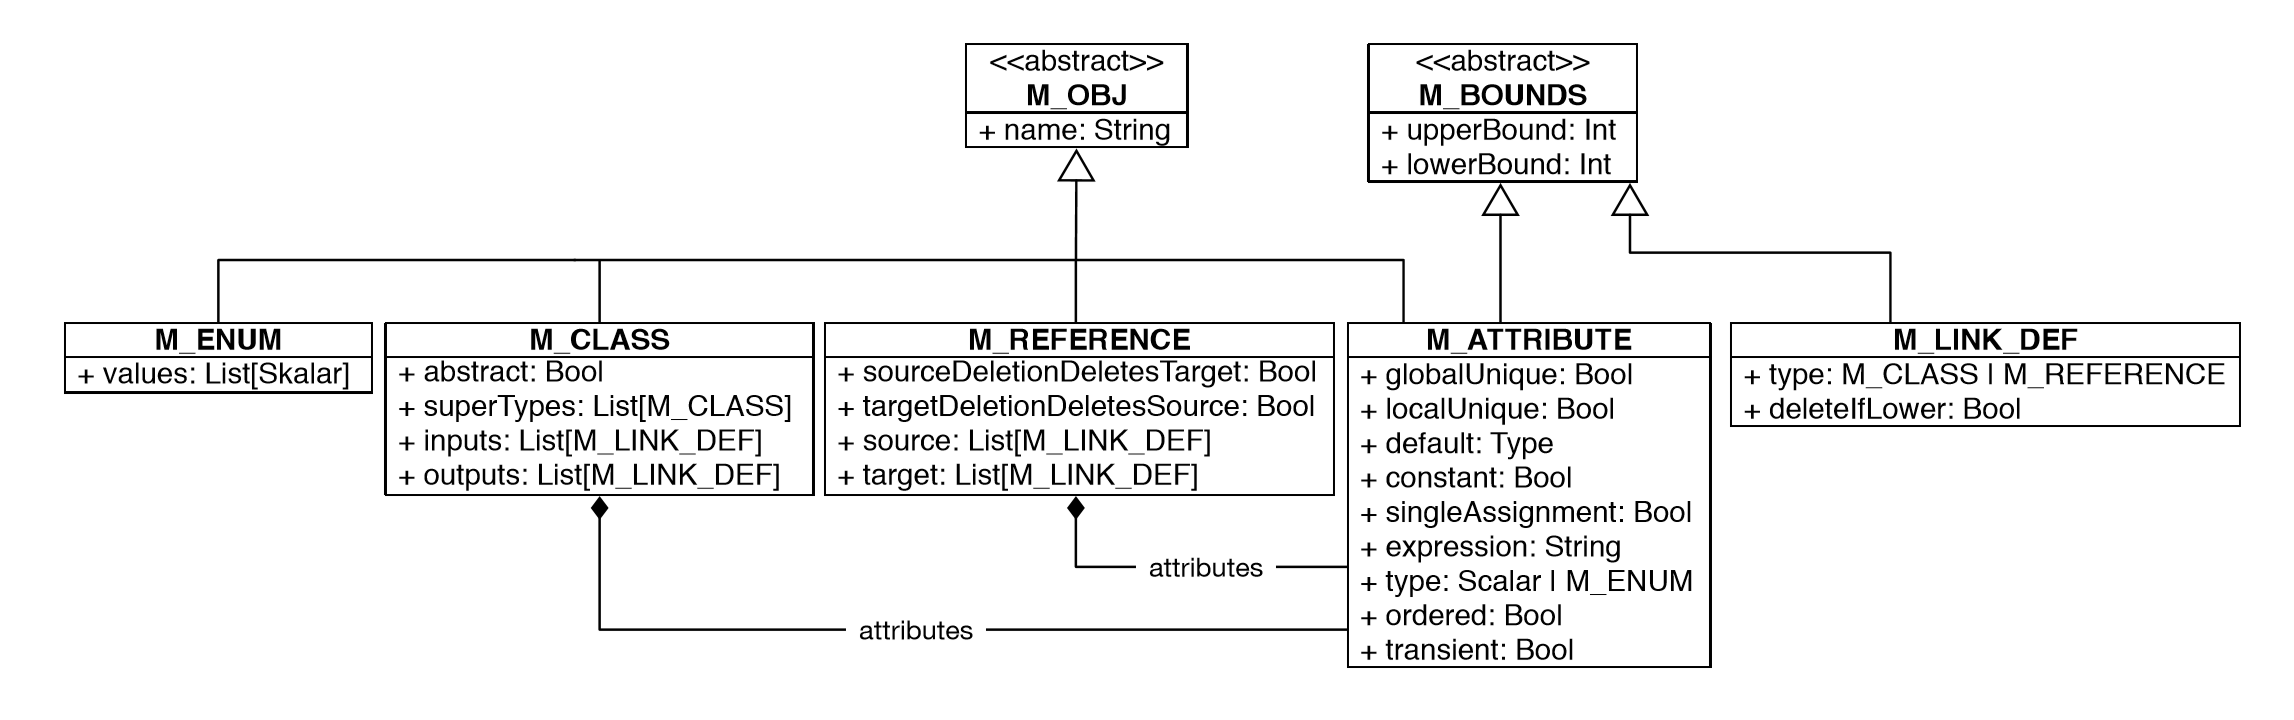
\includegraphics[width=\linewidth]{Abschnitte/Abbildungen/Grafiken/MoDiGen-Metamodel}
%
\epsfig{file=Quadrat.eps,height=1in,width=1in}
\caption{MoDiGen Metamodel}
\label{fig:MoDiGen-Metamodel}
\end{figure*}

Die abstrakte Klasse \textbf{M\_OBJ} enth\"alt das Attribut \textit{name}, dessen Wert innerhalb des gesamten Modells unikat ist. Dadurch wird es m\"oglich die erbenden Objekte zu identifizieren also die Instanzen von \textbf{M\_ENUM}, \textbf{M\_CLASS}, \textbf{M\_REFERENCE} und \textbf{M\_ATTRIBUTE}.
Eine Klasse mit ihren Attributen wird durch \textbf{M\_CLASS} und durch die Komposition zu \textbf{M\_ATTRIBUTE} im Modell erfasst. Vererbung wird durch das Attribut \textit{superTypes} modelliert. Hier ist anzumerken, dass auch Mehrfachvererbung dargestellt werden kann, da eine reflexive * Multiplizität vorliegt. 
Assoziationen werden durch \textbf{M\_LINK\_DEF} modelliert. Jede aus- bzw. eingehende Assoziation einer Klasse wird durch die Attribute \textit{inputs} und \textit{outputs} von \textbf{M\_CLASS} dargestellt, die auf \textbf{M\_LINK\_DEF} zeigen. Der \textit{typ} von \textbf{M\_LINK\_DEF} kann direkt eine \textbf{M\_CLASS} oder eine \textbf{M\_REFERENCE} sein. \textit{deleteIfLower} bestimmt, ob die enthaltende \textbf{M\_CLASS} bzw. \textbf{M\_REFERENCE} gel\"oscht wird sobald \textit{lowerBound} unterschritten wird. Um beliebige Multiplizitäten und Rollen zu beschreiben, wird \textbf{M\_REFERENCE} verwendet. Dazu besitzt diese Klasse die Attribute \textit{source} und \textit{target}, die jeweils beliebig viele Instanzen von \textbf{M\_LINK\_DEF} referenzieren können. Die Attribute \textit{lower-} und \textit{upperBound} von \textbf{M\_LINK\_DEF} bestimmen die Multitplizität. Um Assoziationsklassen \cite{larman2005book}[S. 290] zu modellieren kann \textbf{M\_REF\-ER\-ENCE} beliebig viele Referenzen zu \textbf{M\_ATTRIBUTE} besitzen. \textbf{M\_ENUM} erg\"anzt das Metamodell um Aufz\"ahlungstypen, die \"uber \textit{type} von \textbf{M\_ATTRIBUTE} verwendet werden k\"onnen.

\subsection{Beispiel}
Um das zugrundeliegende JSON-Format n\"aher zu beschreiben, wird im Folgenden als Beispiel ein vereinfachter Familienstammbaum verwendet (siehe Abbildung \ref{fig:Family-Tree-Model}).\\ 
Es existiert eine Entiät \textbf{Person}, die \textit{Vornamen}, \textit{Sozialversicherungsnummer} und \textit{Geburtstag} als Attribute besitzt. Die beiden Klassen \textbf{Male} und \textbf{Female} erben von \textbf{Person} und besitzen keine Attribute. Dabei kann \textbf{Male} eine Assoziation zu \textbf{Female} mit der Rolle \textit{isHusband} haben und, umgekehrt, die Klasse \textbf{Female} zu \textbf{Male} mit der Rolle \textit{isWife}. Das Eltern-Kind verh\"altnis wird durch 1:m Assoziationen von \textbf{Female} bzw. \textbf{Male} zu \textbf{Person} und der dazugeh\"origen Rolle (\textit{isMother}, \textit{isFather}) beschrieben.

\begin{figure}[H]
\centering
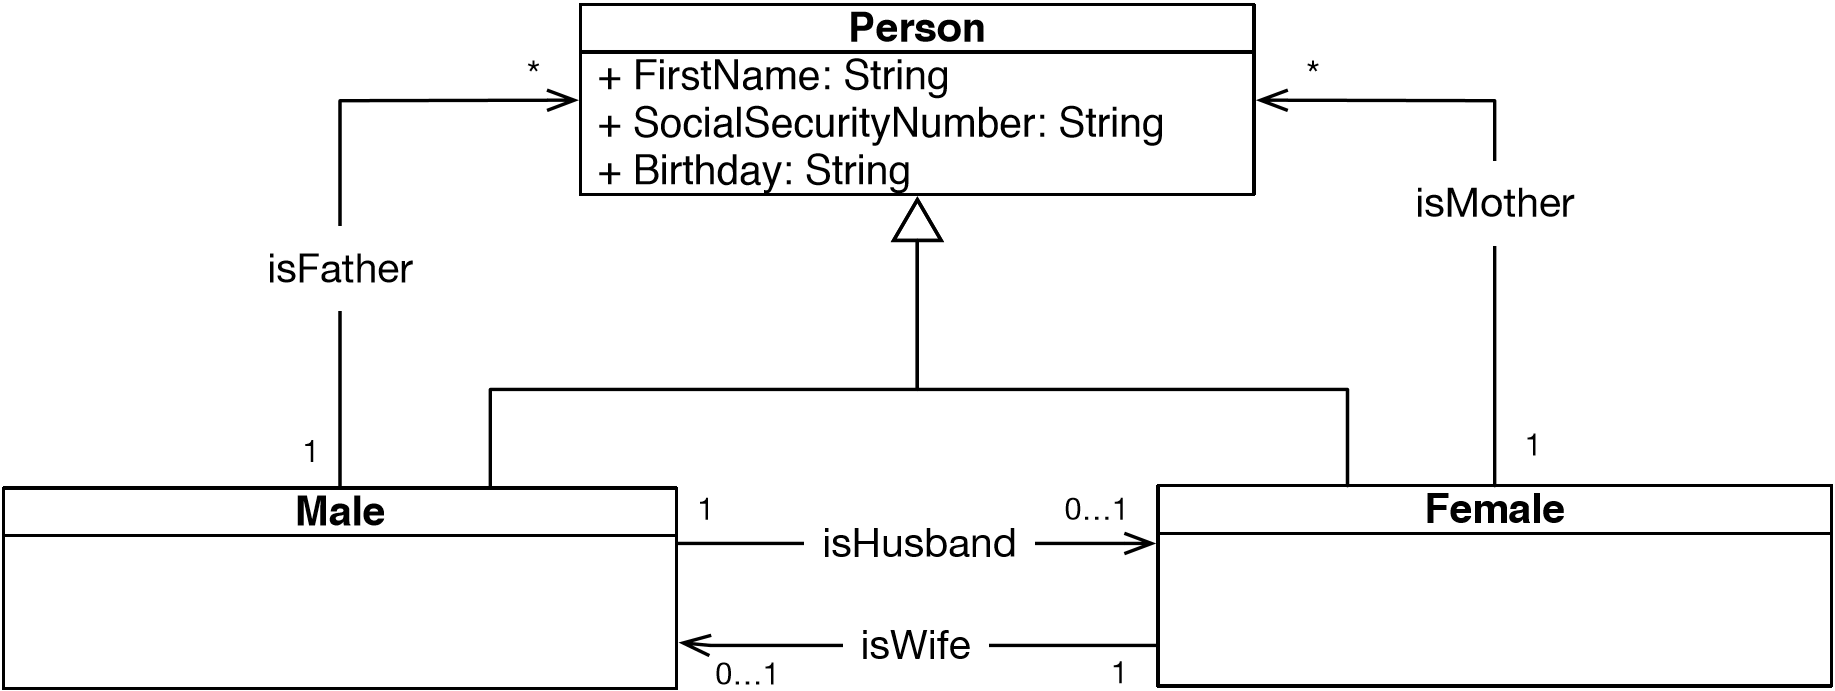
\includegraphics[width=\linewidth]{Abschnitte/Abbildungen/Grafiken/Family-Tree-Model}
\caption{Family Tree Model}
\label{fig:Family-Tree-Model}
\end{figure}


Die Klasse \textbf{Male} kann wie Listing \ref{lst:malejson} zeigt als JSON gespeichert werden. Dabei wird das JSON-Objekt \"uber den Klassennamen identifiziert -- hier \textit{Male} -- und durch das Attribut \textit{mType} als Klasse bestimmt. Da JSON keine implizite Typisierung unterstützt -- es unterscheidet lediglich zwischen wenigen generischen Datentypen -- muss hier explizit festgelegt werden, dass es sich um \textit{mClass} handelt. Die Assoziationen werden entsprechend als JSON-Arrays \textit{inputs} und \textit{outputs} gespeichert und enthalten die durch \textbf{M\_LINK\_DEF} definierten Attribute.

\lstlistingCode{M\_CLASS Male aus dem Family Tree Beispiel}{malejson}
"Male": { 
  "mType": "mClass", 
  "name": "Male",
  "superTypes": ["Person"], 
  "mAttributes": [], 
  "inputs": [{ 
    "type": "isWife", 
    "upperBound": 1, 
    "lowerBound": 0 
  }], 
  "outputs": [{ 
    "type": "isHusband", 
    "upperBound": 1,
    "lowerBound": 0 
    },{ 
    "type": "isFather", 
    "upperBound": -1,
    "lowerBound": 0
  }] 
}
\end{lstlisting}

Eine \textbf{M\_REFERENCE} wird als "`Objekt erster Klasse"' gespeichert wie Listing \ref{lst:ishusbandjson} zeigt und kann damit unabhängig von den \textbf{M\_CLASS} instanzen geladen werden. Das JSON-Objekt wird durch den Namen der \textbf{M\_REFERENCE} identifiziert und enth\"alt alle Attribute. Der Typ wird hier, wie bei \textbf{M\_CLASS} instanzen in \textit{mType} abgelegt. In den JSON-Arrays \textit{source} und \textit{target} werden, genau wie bei den \textbf{M\_CLASS} instanzen, die gesamten \textbf{M\_LINK\_DEF} instanzen abgelegt. In diesem Modell kann \textbf{Male} eine Assoziation der Rolle \textit{isHusband} haben. Diese \textbf{M\_LINK\_DEF} instanz zeigt auf die entsprechende \textbf{M\_REFERENCE} instanz, die wiederrum mit zwei Endpunkten zu \textbf{Female} und \textbf{Male} existiert. \textit{upper-/lowerBounds} sind hier jeweils 1, also wird der Sachverhalt "`Ein Ehemann ist der Mann einer Frau"' modelliert.

\lstlistingCode{Husband M\_REFERENCE Male aus dem Family Tree Beispiel}{ishusbandjson}
"isHusband": {
  "mType": "mRef", 
  "name": "isHusband",
  "mAttributes": [], 
  "source": [{ 
    "type": "Male", 
    "upperBound": 1, 
    "lowerBound": 1 
  }], 
  "target": [{ 
    "type": "Female", 
    "upperBound": 1, 
    "lowerBound": 1, 
  }] 
} 
\end{lstlisting}

Die Instanzen werden durch UUIDs identifiziert und enthalten Verweise auf ihre Typen im Modell sowie ihre Typen im Metamodell. Dies ist z.B durch die Kombination \textit{"`mClass"': "`Male"'} in Zeile 2 von Listing \ref{lst:instancejson} zu sehen. Es handelt sich um eine Instanz von \textbf{Male}, die wiederrum als Klasse, also als Instanz von \textbf{M\_CLASS} modelliert ist. Die \textit{outputs} und \textit{inputs} verweisen hier auf Instanzen von konkreten Referenzen -- in diesem Fall \textit{isHusband}, \textit{isWife} und \textit{isFather}.\\
Die Referenz \textit{isHusband} zeigt gem\"a\ss des Modells (Abbildung \ref{fig:Family-Tree-Model}) in \textit{source} auf eine Instanz von \textbf{Male} und in \textit{target} auf eine Instanz von \textbf{female}.

\lstlistingCode{Family Tree Instanz}{instancejson}
"846bc8a2-00fc-401f-b626-0b0252516aee": { 
  "mClass": "Male", 
  "outputs": { 
    "isFather": 
      ["8e9b1093-a589-4ae4-8e1e-1b3d63a3f842"], 
    "isHusband": 
      ["ee204744-6322-49d4-928e-1442e8bc70c4"] 
  }, 
  "inputs": { 
    "isWife": 
      ["666d4de7-e0f2-4620-8c19-d5469b40be1f"] 
  }, 
  "mAttributes": { 
    "First_Name": ["Hans"], 
    "SocialSecurityNumber": ["12"], 
    "Birthday": ["12-02-2015"] 
  } 
}, 

"ee204744-6322-49d4-928e-1442e8bc70c4": { 
  "mRef": "isHusband", 
  "source": { 
    "Male": 
      ["846bc8a2-00fc-401f-b626-0b0252516aee"] 
  }, 
  "target": { 
    "Female": 
      ["a264a43b-6f97-4257-9243-baddbf745490"] 
  } 
} 
\end{lstlisting}

\begin{figure}[H]
\centering
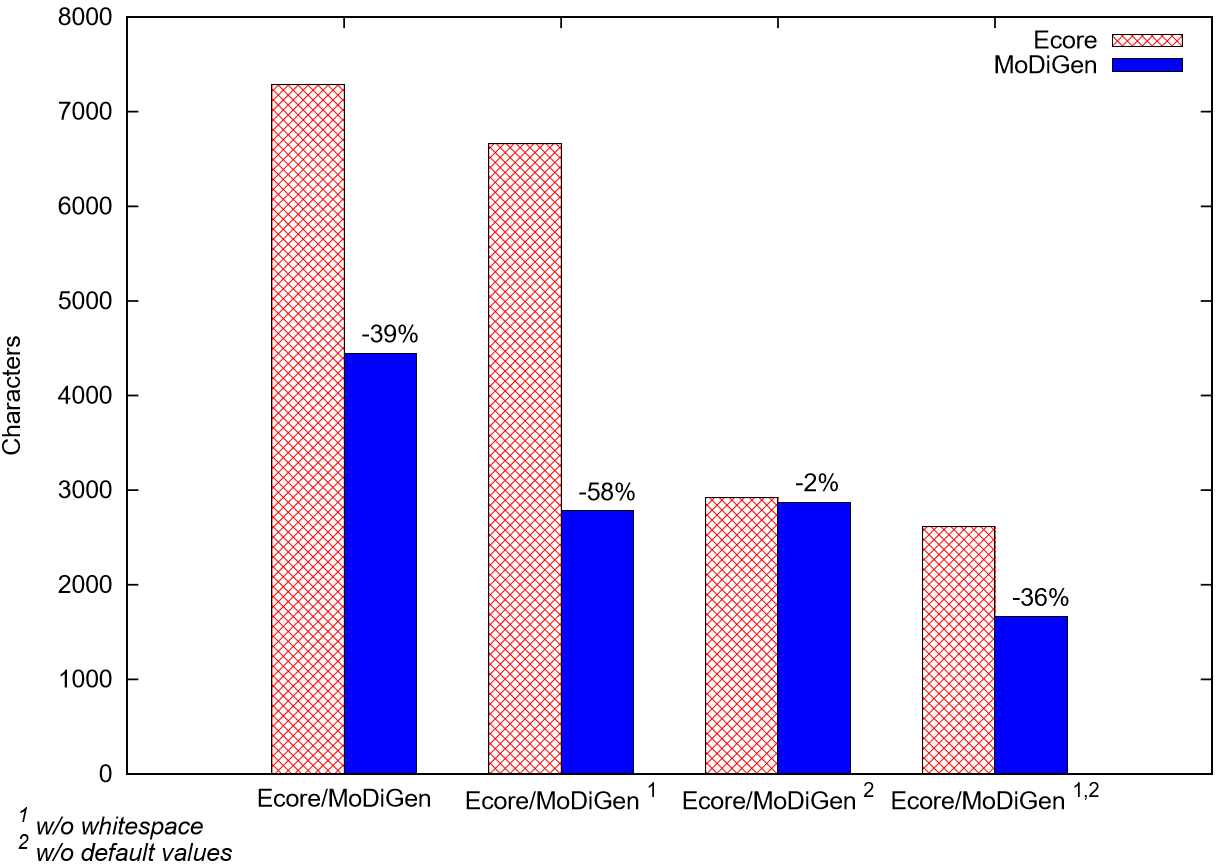
\includegraphics[width=\linewidth]{Abschnitte/Abbildungen/Grafiken/Num-Char-Family-Tree-Model}
\caption{Buchstabenanzahlvergleich aus dem Family Tree Beispiel}
\label{fig:Num-Char-Family-Tree-Model}
\end{figure}

\begin{figure}[H]
\centering
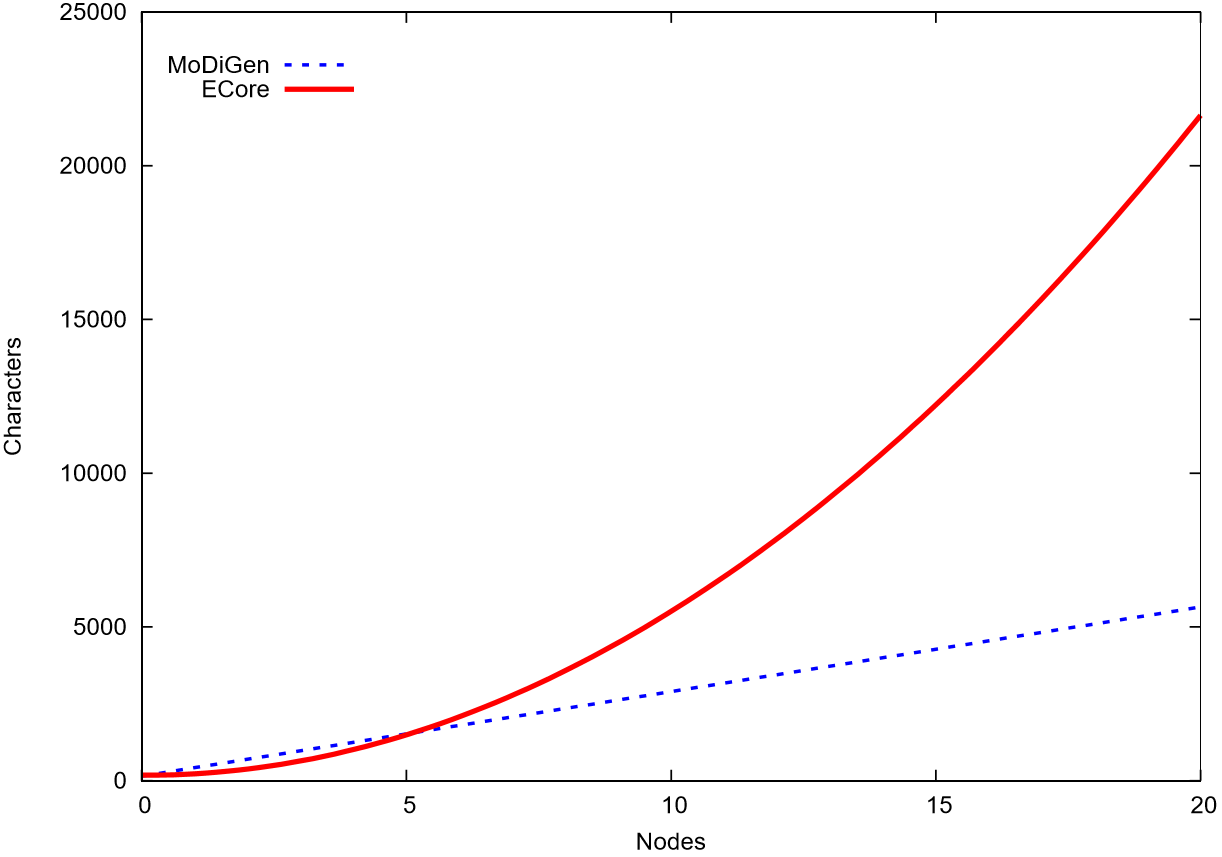
\includegraphics[width=\linewidth]{Abschnitte/Abbildungen/Grafiken/Characters-and-Nodes}
\caption{Buchstabenmenge im Verhältnis zu erzeugten Knotenpunkte}
\end{figure}








